\documentclass[10pt, unicode, xcolor={svgnames, table, hyperref}]{beamer}


\usetheme{Default}



%\usetheme[progressbar=frametitle,titleformat=smallcaps,sectionpage=none,numbering=fraction]{metropolis}
%\setbeamerfont{frametitle}{size=\normalsize}
\setbeamerfont{frametitle}{size=\large}
\usepackage[framemethod=default]{mdframed}
% цветовая схема

% пакет для рамочек у определения
\usepackage[many]{tcolorbox}
\usepackage{geometry}

% чтобы заголовок слайда был по центру
\setbeamertemplate{frametitle}[default][center]

\newtcolorbox{defin}{colback=blue!8, rightrule=0pt, toprule=0pt, bottomrule=0pt,
					 skin=enhancedlast jigsaw, arc=0mm, colframe=blue!40}
% As well as themes, the Beamer class has a number of color themes
% for any slide theme. Uncomment each of these in turn to see how it
% changes the colors of your current slide theme.

%\addtolength{\headsep}{0.6cm}
\setbeamertemplate{footline}[page number]

%\usecolortheme{default}
%\usecolortheme{albatross}
%\usecolortheme{beaver}
%\usecolortheme{beetle}
%\usecolortheme{crane}
%\usecolortheme{dolphin}
%\usecolortheme{dove}
%\usecolortheme{fly}
%\usecolortheme{lily}
%\usecolortheme{orchid}
%\usecolortheme{rose}
%\usecolortheme{seagull}
%\usecolortheme{seahorse}
%\usecolortheme{spruce}
%\usecolortheme{whale}
%\usecolortheme{wolverine}

%beaver modifications
%\setbeamercolor{title}{bg=Gainsboro,fg=DarkRed}
%\setbeamercolor{frametitle}{bg=WhiteSmoke,fg=DarkRed}

\setbeamercolor{math text}{fg=DarkBlue!80!LightBlue}

%\setbeamercolor{block title}{bg=LightGray,fg=DarkRed}
%\setbeamerfont{block title}{series=\bfseries} 
%\setbeamercolor{block body}{bg=WhiteSmoke}
%\setbeamerfont{block body}{shape=\itshape}

%for metropolis
%\setbeamercolor{normal text}{bg=white,fg=black}
%\setbeamercolor{title}{bg=white,fg=NavyBlue}
%\setbeamercolor{frametitle}{bg=NavyBlue,fg=white}
%\setbeamercolor{progressbar}{bg=Blue,fg=white}

%ПРЕАМБУЛА
%основное
\usepackage{cmap} % для кодировки шрифтов в pdf
\defaulthyphenchar=127 
\usepackage[T1,T2A]{fontenc} 
\usepackage[utf8]{inputenc}
\usepackage[english,russian]{babel}

%\usepackage{indentfirst}\parindent=2.5em 

%математика
\usepackage{amsmath,amstext,amsfonts,amssymb}
\usepackage{mathtext,mathrsfs,array}

\usepackage{moreverb}

%% Выбор шрифтов %% 

%\usepackage{mathptmx}
%\usepackage{helvet} %arev, avant, bookman, chancery, charter, euler, helvet, lmodern,mathtime ,mathptm, mathptmx, newcent, palatino, pifont, utopia.
%\usepackage{bookman}

%\usefonttheme{serif} % нормальные шрифты текста-формул в целом
\usefonttheme{professionalfonts} % все sffamily кроме формул (они serif)
%\usepackage{concmath}
%\usepackage{cmbright}
%\usefonttheme[stillsansserifmath]{serif}
%\usefonttheme[onlymath]{serif} % Использовать шрифт с засечками для формул (+ \usepackage{cmbright} --- хорого отображаются гречиские буквы)
%\usefonttheme[onlylarge]{structurebold} % main , frame titles, and section entries in the table of contents будут жирненькими
%\setbeamerfont{institute}{size=\normalsize} % Более крупный шрифт для подзаголовков титульного листа

%\setbeamerfont{title}{family=\sffamily}%,size=\large
%\setbeamerfont{subtitle}{family=\sffamily,size=\small}
\setbeamerfont{author}{size=\normalsize}
%\setbeamerfont{institute}{size=\normalsize}
\setbeamerfont{date}{size=\normalsize}
%\setbeamerfont{frametitle}{family=\sffamily}
%\setbeamerfont{block title}{family=\sffamily,size=\large}
%\setbeamerfont{contents}{family=\sffamily}

%\setbeamerfont{bibliography item}{size=\small}
%\setbeamerfont{bibliography entry author}{shape=\itshape}
%\setbeamerfont{bibliography entry title}{size=\small}
%\setbeamerfont{bibliography entry location}{size=\small}
%\setbeamerfont{bibliography entry note}{size=\small}

\useinnertheme{circles}
%\useinnertheme{rectangles}


\usepackage{soulutf8}% Поддержка переносоустойчивых подчёркиваний и зачёркиваний
\usepackage{icomma}  % Запятая в десятичных дробях

%%%%%%%%%%%%%%%%%%%

% Если используется последовательное появление пунктов списков на
% слайде (не злоупотребляйте в слайдах для защиты дипломной работы),
% чтобы еще непоявившиеся пункты были все-таки немножко видны.
\setbeamercovered{transparent}

% отключить клавиши навигации
\setbeamertemplate{navigation symbols}{}

%command to set the logo to nothing
\newcommand{\nologo}{\setbeamertemplate{logo}{}} 


\usepackage{comment}  %для комментирования большого крол-ва строк

\newcommand{\specialcell}[2][c]{% объявляем новую команду для переноса строки внутри ячейки таблицы
	\begin{tabular}[#1]{@{}c@{}}#2\end{tabular}}

%гафика 
\usepackage{pgf,tikz,pgfplots}
\pgfplotsset{compat=1.15}
\usepackage{tcolorbox}
\usetikzlibrary{arrows,arrows.meta,patterns,shadings,shadows}
\tcbuselibrary{skins,breakable}
%\usepackage{multicol}
%\usepackage{csquotes}

% это чтобы вставлять источники под фото
\usepackage{stackengine}
\usepackage{url}

\usepackage{tabularx}



%\usepackage{footmisc}
%\renewcommand{\thefootnote}{}

%++++++++++++++++++++++++++++++++++++++++++++++++++++++++++++++++++++++++++++++++++++++++++++++++++++++++++++++++++++++++++++



%\title{Статистический анализ численности населения РФ}

%\subtitle{КУРСОВАЯ РАБОТА}

%\author{Кирякин Максим Валерьевич}

%\institute{\normalsize МГУ им. М. В. Ломоносова\\ Кафедра вычислительных технологий и моделирования}

%\date{\today}

%\logo{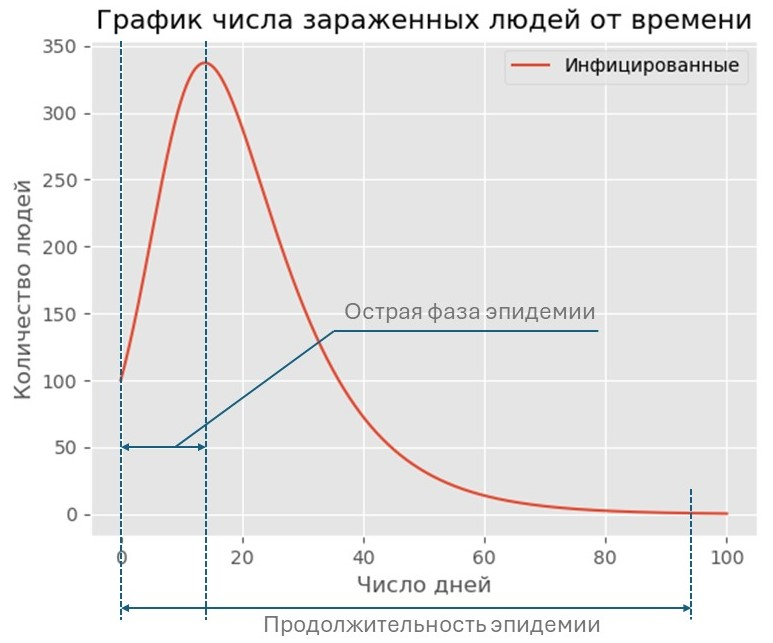
\includegraphics[width=0.15\textwidth]{img/1.png}}


% for easy using in mathematics formula 

%\usepackage{autonum}
%\input{math_redef} 
%\newcommand{\grad}{\operatorname{grad}}
%\newcommand{\rot}{\operatorname{rot}}
%\renewcommand{\div}{\operatorname{div}}

% нумерация рисунков
\setbeamertemplate{caption}[numbered]
%=======================================
\setlength{\parindent}{0pt}

% выравнивает текст по ширине
\usepackage{ragged2e}
\justifying

\begin{document}
	
	

% Создание заглавной страницы

\setbeamerfont{title}{size=\large}
\setbeamerfont{subtitle}{size=\small}
\setbeamerfont{author}{size=\large}
\setbeamerfont{date}{size=\small}
%\setbeamersize{text margin left=0.5cm, text margin right=0.5cm}
\setbeamerfont{institute}{size=\small}
\title[Дипломная работа]{\textbf{Применение компартментно-сетевых моделей \\ для моделирования эпидемического процесса } \\ }

\institute
{
Научный руководитель:
д.ф.-м.н., профессор Романюха А.А.
\and
Со-руководитель:
к.ф.-м. н. Санникова Т.Е.
}

\author[Кирякин М. В.]{Кирякин М. В.}

\date[\textcolor{white}{20 Мая, 2024} ]{20 Мая, 2024} 


\frame{\titlepage} 



\setlength{\parskip}{0pt} % установка расстояния между пунктами оглавления



% Автоматическая генерация содержания

%\begin{frame}{Содержание}
%\tableofcontents
%\end{frame}

\section{Цель и задачи работы}
\begin{frame}[t]{Цель и задачи работы}

	\textbf{Цель}: Исследование влияния свойств сети контактов на динамику эпидемиологического процесса при помощи компартментно-сетевой модели.
	
	\vspace{0.5cm}
	  
	\textbf{Задачи:}
	\begin{enumerate}
		\item Разработать алгоритм построения сети контактов для жителей городской и сельской местностей на основе демографических и социо-эконономических данных о населении Российской Федерации.
		
		\item  Реализовать компартментно-сетевую модель для описания распространения респираторной инфекции в популяциях городского и сельского типов.
		
		\item Промоделировать распространение инфекции в популяциях с различными типами сетей контактов.
	\end{enumerate}
\end{frame}
		
\section{Теоретические аспекты решения задачи моделирования распространения инфекции}
\begin{frame}[fragile,t]{Теоретические аспекты решения задачи моделирования распространения инфекции}
	
	\begin{defin}
		\textbf{Определение}.
		Под эпидемически значимый контактом будем понимать социальный контакт, при котором возможна передача респираторной инфекции.
	\end{defin}	

	\begin{defin}
		\textbf{Определение}.
		Сеть контактов -- неориентированный граф $G(N, V)$, где $N$ - количество вершин, а $V$ - количество ребер. Каждая вершина соответствует члену популяции, а ребро между вершинами $i$ и $j$ ($i,j \in \overline{1, N}$) существует в том и только том случае, если между $i$-м и $j$-м индивидом имеет место эпидемически значимый контакт в течение дня хотя бы 5 дней из 7.
	\end{defin}	

	Основные подходы к созданию сетей контактов:
	\begin{enumerate}
		\item  Использование данных о реальной популяции (Например, использование опросников)
		\item  Использование математических моделей (Например, модель <<малого мира>>, безмасштабные сети)
	\end{enumerate}

\end{frame}

\begin{frame}[fragile,t]{}

	\begin{defin}
		\small
		\textbf{Определение}.
		Компартментными называются модели, которые предполагают, что популяция разделяется на субпопуляции (компартменты) в соответствии с их инфекционным статусом.
		
	\end{defin}	

	\begin{defin}
		\small
		\textbf{Определение}.
		Компартментно-сетевыми называются модели, в которых популяция разделяется на различные субпопуляции (компартменты) в соответствии с их инфекционным статусом и числом контактов. Являются развитием компартментных моделей.
	\end{defin}	

	\begin{defin}
		\small
		\textbf{Определение}.
		Эпидемия -- это быстрое распространение
		заболевания среди людей, превышающее обычный уровень заболеваемости на данной территории.
	\end{defin}	
		
	\begin{defin}
		\small
		\textbf{Определение}.
		Острая фаза эпидемии -- это период времени, в течение которого наблюдается резкий рост функции числа инфицированных.
	\end{defin}		
		
	
\end{frame}
	

\begin{comment}
\begin{frame}[fragile,t]{}
	
	\vspace{0.5cm}
	\textcolor{DarkBlue!80!LightBlue}{1.2 SIR модель}
	\vspace{0.2cm}
	
	Модель описывается системой дифференциальных уравнений \eqref{eq:SIR_system_base}.
	\begin{equation}
		\begin{cases}
			\frac{d S}{d t} = -\beta  I S, \\
			\frac{d I}{d t} = -\mu I + \beta  I S, \\
			\frac{d R}{d t} = \mu I .
		\end{cases}
		\label{eq:SIR_system_base}
	\end{equation}
	
	\begin{itemize}
		
		\item $S(t)$ -- доля людей, которые могут заразиться инфекцией.
		\item $I(t)$ -- доля людей, которые в текущий момент времени заражены и могут распространять инфекцию.
		\item $R(t)$ -- доля людей, которые обладают иммунитетом к болезни, так как недавно переболели или были вакцинированны.
		\item $\beta$, $\mu$ -- скорость распространения инфекции, скорость выздоровления человека соответственно. 
		
	\end{itemize}
	
	При этом предполагается, что все три величины в любой момент времени удовлетворяют условию:
	
	\begin{equation}
		S(t) + I(t) + R(t) = 1
		\label{eq:norm}
	\end{equation}

\end{frame}
\end{comment}



\begin{frame}[fragile,t]{}
	Введем обозначения:
	\begin{itemize}
	
		\item $S_k(t)$, $S(t)$ -- доля узлов степени k, восприимчивых в момент времени t; общая доля восприимчивых узлов в момент времени t
		\item$I_k(t)$, $I(t)$ -- доля узлов степени k, инфицированных в момент времени t; общая доля инфицированных узлов	в момент времени t.
		\item $R_k(t)$, $R(t)$ -- доля узлов степени k, выздоровевших в момент времени t; общая доля выздоровевших узлов, в момент времени t.
		\item $\lambda_k$ -- вероятность, с которой узел степени k может быть заражен, если у него есть общие ребра с инфицированными узлами.
		\item $\beta_0$ -- это постоянная скорость, с которой происходит заражение восприимчивых узлов.
		\item $\mu$ -- постоянная скорость, с которой инфицированные узлы выздоравливают.
	
	\end{itemize}

	Значение $k$ изменяется от 1 и ограничивается количеством уникальных степеней вершин в графе, формирующем сеть контактов.
\end{frame}




\begin{frame}[fragile,t]{}
	
	\vspace{0.5cm}
	\textcolor{DarkBlue!80!LightBlue}{Модель гетерогенного перемешивания}
	\vspace{0.2cm}
	
    Модель гетерогенного перемешивания\footnote{Moreno Y., Pastor-Satorras R., Vespignani A. Epidemic outbreaks in complex heterogeneous networks //The European Physical Journal B-Condensed Matter and Complex Systems. – 2002. – Т. 26. – С. 521-529}.  основана на динамической структуре, учитывающей степени вершин в сети
	контактов.
	
	\begin{equation}
		\begin{cases}
			\frac{d S_k}{d t} = -\lambda_k \beta_0 S_k \Theta(t), \\
			\frac{d I_k}{d t} = -\mu I_k + \lambda_k \beta_0 S_k \Theta(t), \\
			\frac{d R_k}{d t} = \mu I_k \\
			\Theta(t)=\cfrac{\sum_{k} k \lambda_{k} I_{k}(t)}{\sum_{k} k \lambda_{k}} \\
			S(t)=\sum_{k} S_{k} \\
			I(t)=\sum_{k} I_{k} \\
			R(t)=\sum_{k} R_{k} \\
			S_k(t) + I_k(t) + R_k(t) = 1
		\end{cases}
		\label{eq:SIR_system_base_groups}
	\end{equation}

	
\end{frame}




\begin{frame}[fragile,t]{Сбор и обработка данных для городской и сельской местностей}

	\begin{figure}[h!]
		\centering
		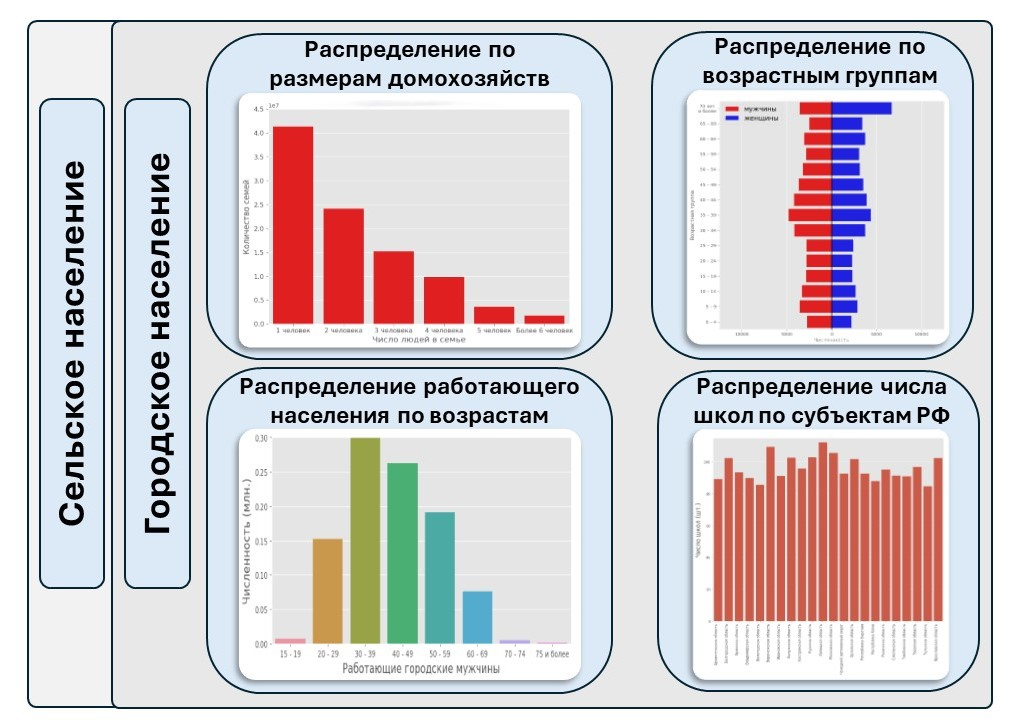
\includegraphics[width=0.95\textwidth]{img/данные.jpg}
		\label{fig:data}
	\end{figure}
	Распределение данных, использованные при создании синтетической популяции.
	
\end{frame}


\section{\small Алгоритм}

\begin{frame}[fragile,t]{Алгоритм создания сети контактов}
	\begin{figure}[h!]
		\centering
		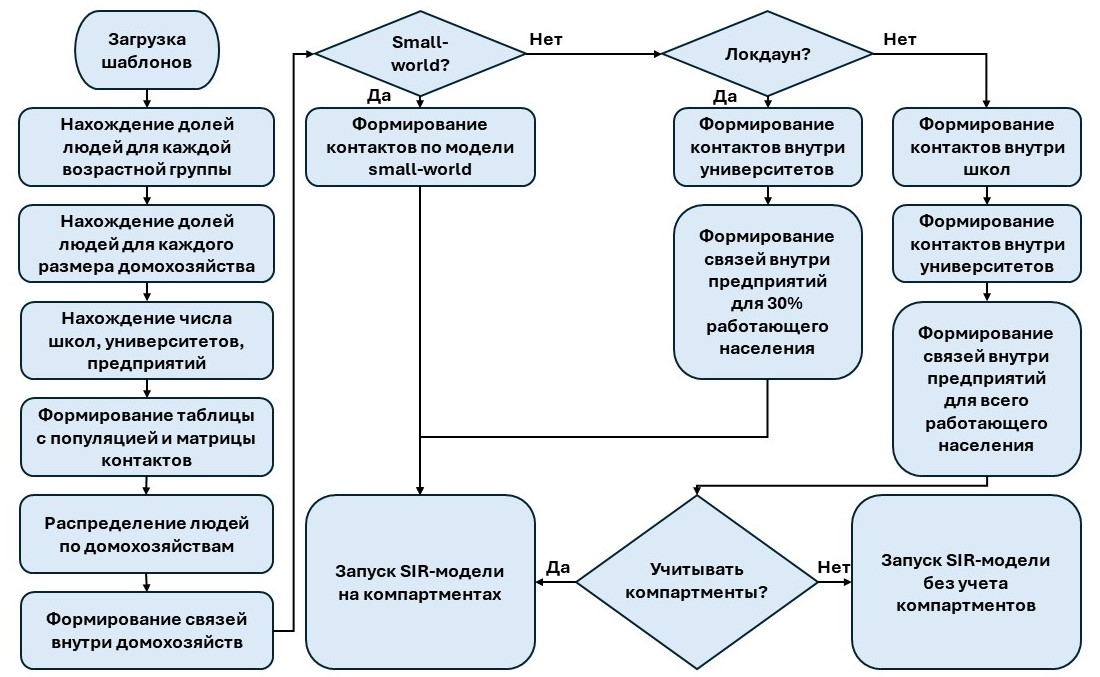
\includegraphics[width=1.0\textwidth]{img/Алгоритм.jpg}
		\label{fig:algo}
		
	\end{figure}
Блок-схема работы алгоритма моделирования распространения инфекции.
\end{frame}

\section{\small Программная реализация алгоритма алгоритма}
\begin{frame}[fragile]{Программная реализация алгоритма создания сети контактов}

	\begin{figure}[h!]
		\begin{minipage}{0.49\textwidth}
			\small
			Для проведения численного моделирования была разработана компьютерная
			программа.
			
			Основные характеристики:
			\begin{enumerate}
				\item язык программы -- Python
				\item 1500 строк кода
				\item 4 программных модуля
				\begin{itemize}
					\item Модуль загрузки данных.
					\item Модуль создания сети контактов.
					\item Расчётный модуль.
					\item Модуль графического интерфейса.
				\end{itemize}
				
			\end{enumerate}
		\end{minipage}
		\begin{minipage}{0.48\textwidth}

			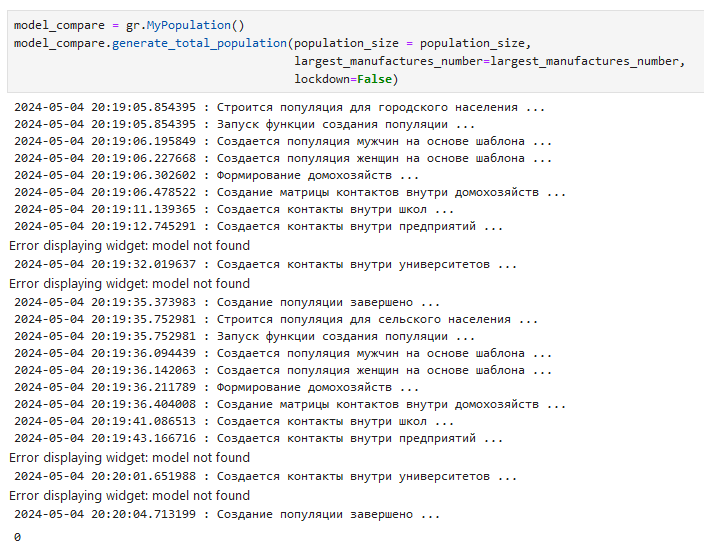
\includegraphics[width=1.\textwidth]{img/прога.png}
			Пример работы программы по созданию искусственной популяции.
		\end{minipage}
	\end{figure}
	Программный код  обеспечивает
	возможность его развития и использования в качестве расчётного модуля в разных современных программных комплексах.
	
\end{frame}




\section{\small Эксперименты}
\begin{frame}[fragile,t]{Эксперименты}

	\textcolor{DarkBlue!80!LightBlue}{Метрики, использованные при моделировании}

	\begin{figure}[h!]
		\begin{minipage}{0.4\textwidth}
		
			\begin{itemize}
				\item Максимальная по всем компартментам время наличия инфекции в популяции.
				\item Средневзвешенное по размерам компартментов значение продолжительности острой фазы инфекции.
				\item Процент переболевших людей.
			\end{itemize}
		\end{minipage}
		\begin{minipage}{0.58\textwidth}

			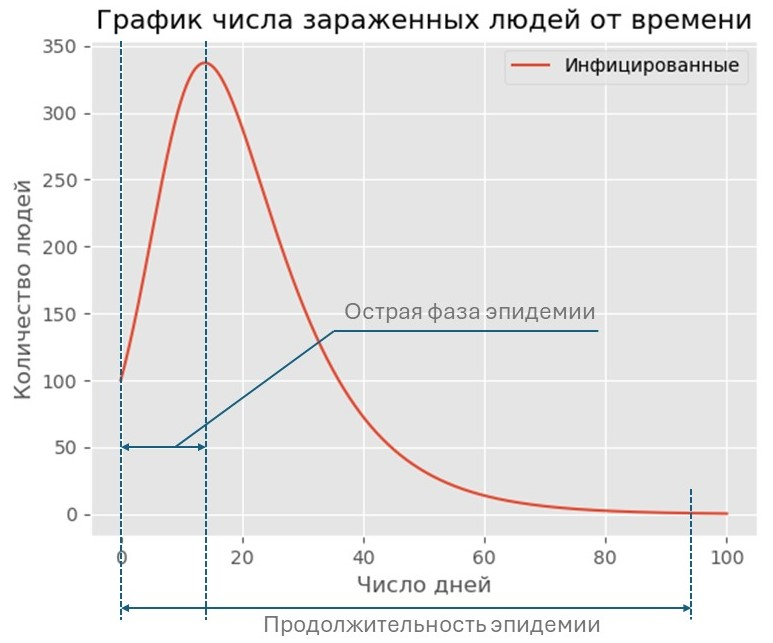
\includegraphics[width=1.\textwidth]{img/1.jpg}

			Описание метрик, пользованных при моделировании динамики распространения инфекции.

		\end{minipage}
		\label{fig:disease_spreading_urban}	
	\end{figure}
	

\end{frame}

\begin{frame}{Моделирование динамики распространения инфекции с помощью SIR модели без учета компартментов}
	
	\begin{figure}[h!]
		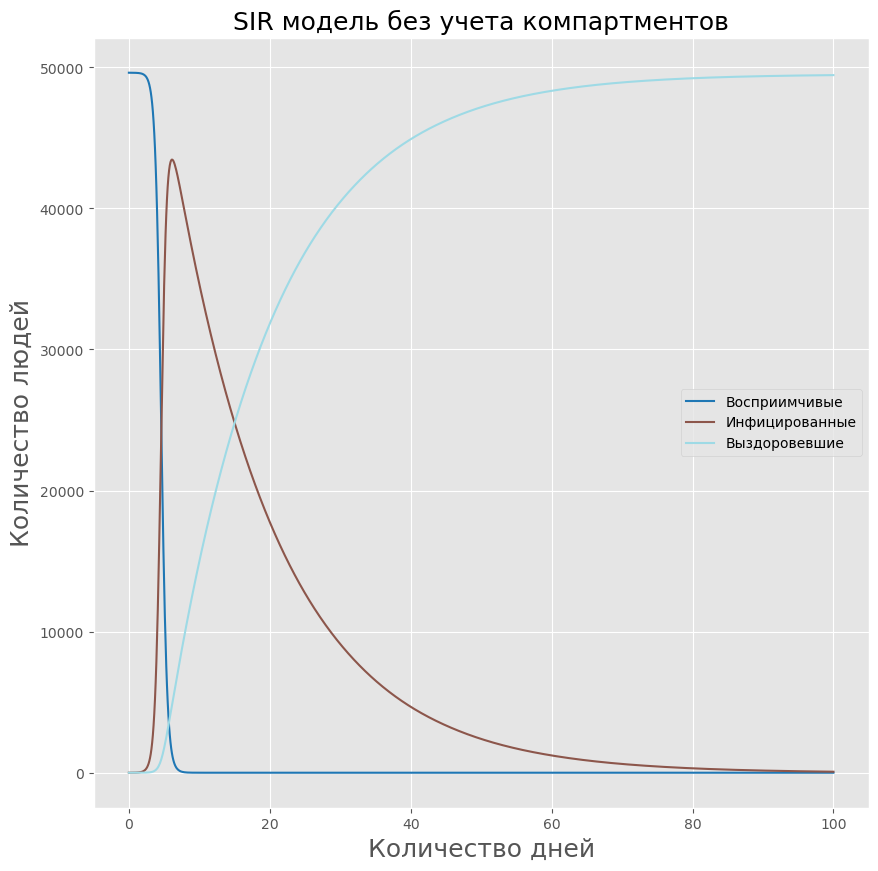
\includegraphics[width=0.6\textwidth]{img/sir_to_all.png}
	\end{figure}
	Динамика изменения численности групп выздоровевших, инфицированных и восприимчивых для модели,	примененной ко всей популяции.
\end{frame}


\begin{frame}{Моделирование динамики распространения инфекции с помощью SIR модели без учета компартментов}
	
	\begin{figure}[h!]
		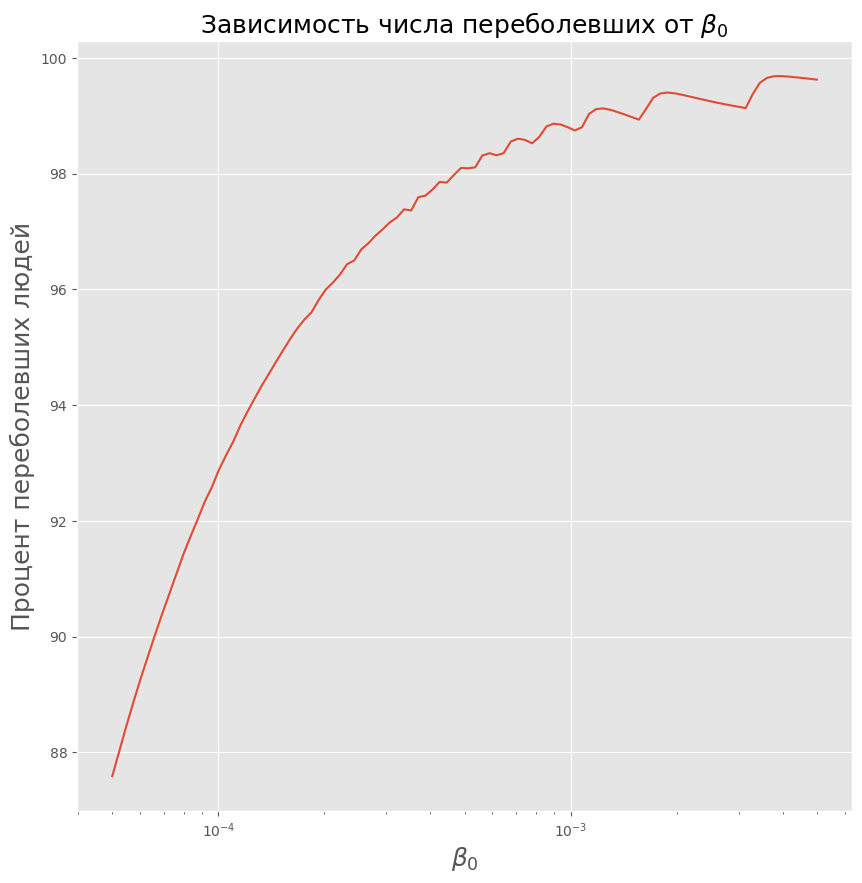
\includegraphics[width=0.6\textwidth]{img/sir_beta.png}
	\end{figure}
	График зависимости процента переболевших людей от скорости распространения инфекции.
	
\end{frame}



\begin{frame}{Сравнение динамики распространения инфекции для сельского и городского населений}
	
	\begin{figure}[h!]
		\begin{minipage}{0.49\textwidth}
			\centering
			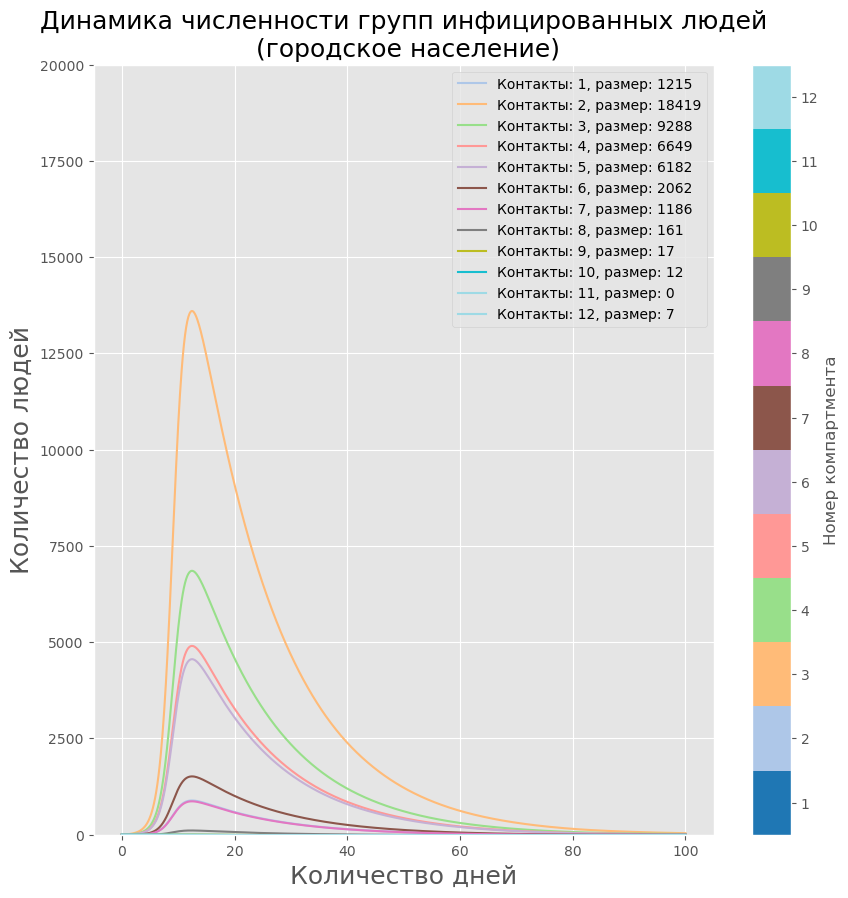
\includegraphics[width=1.0\textwidth]{img/sir_model_compare_I_urban_new.png}
		\end{minipage}
		\begin{minipage}{0.49\textwidth}
			\centering
			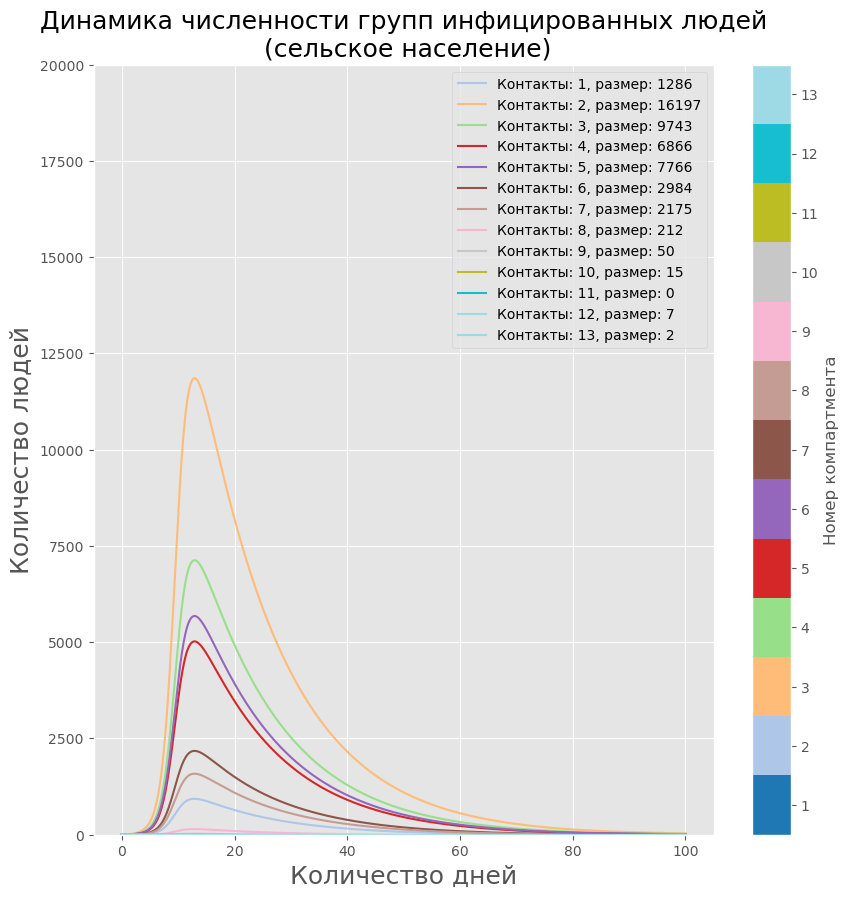
\includegraphics[width=1.0\textwidth]{img/sir_model_compare_I_rural_new.png}
		\end{minipage}
	\end{figure}
	Динамика изменения численности групп инфицированных и выздоровевших людей с течением времени для городского населения.
	
\end{frame}


\begin{frame}{Моделирование динамики распространения инфекции при условии локдауна}
	
	\begin{figure}[h!]
		\begin{minipage}{0.49\textwidth}
			\centering
			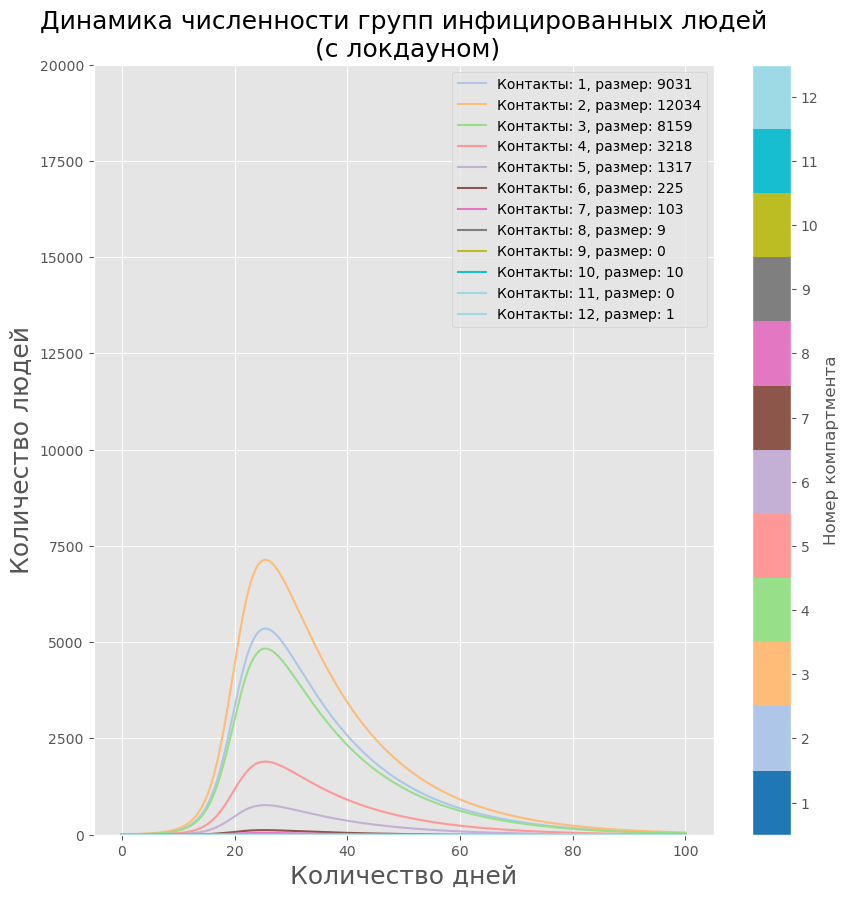
\includegraphics[width=1.0\textwidth]{img/sir_model_lockdown_urban_I_new.png}
		\end{minipage}
		\begin{minipage}{0.49\textwidth}
			\centering
			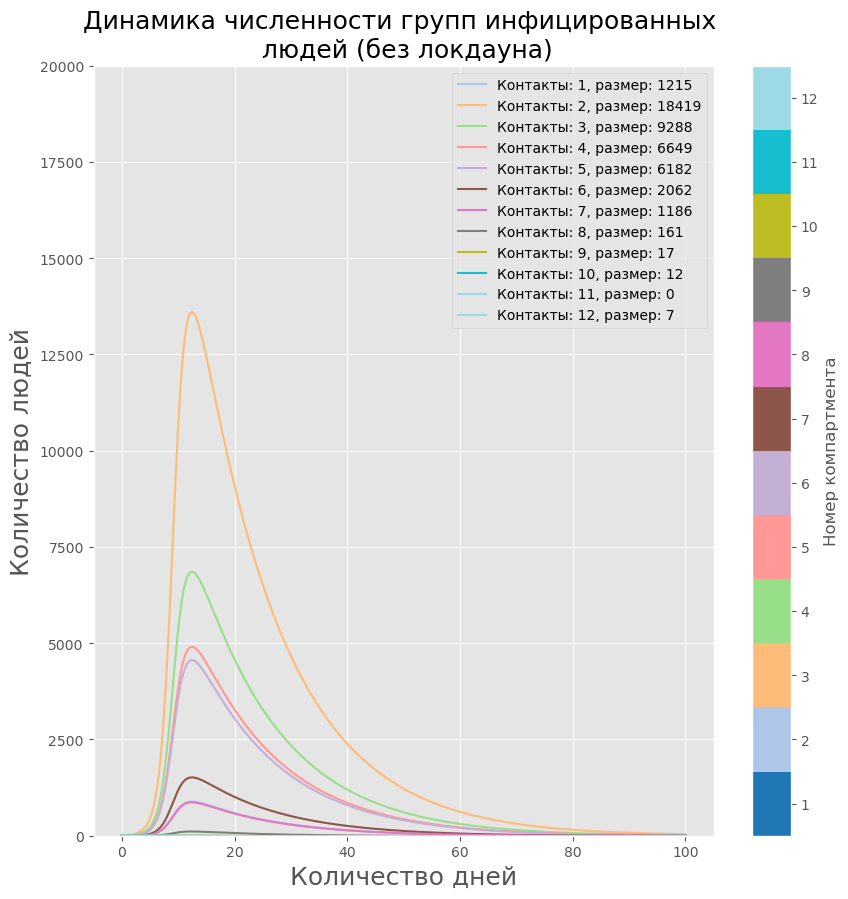
\includegraphics[width=1.0\textwidth]{img/sir_model_nonlockdown_urban_I_new.png}
		\end{minipage}
	\end{figure}
	Динамика изменения численности групп инфицированных людей с течением времени
	при наличии локдауна и без него.
\end{frame}


\begin{frame}{Моделирование динамики распространения инфекции на сети контактов, построенной по методу small-world}
	
	\begin{figure}[h!]
		\begin{minipage}{0.49\textwidth}
			\centering
			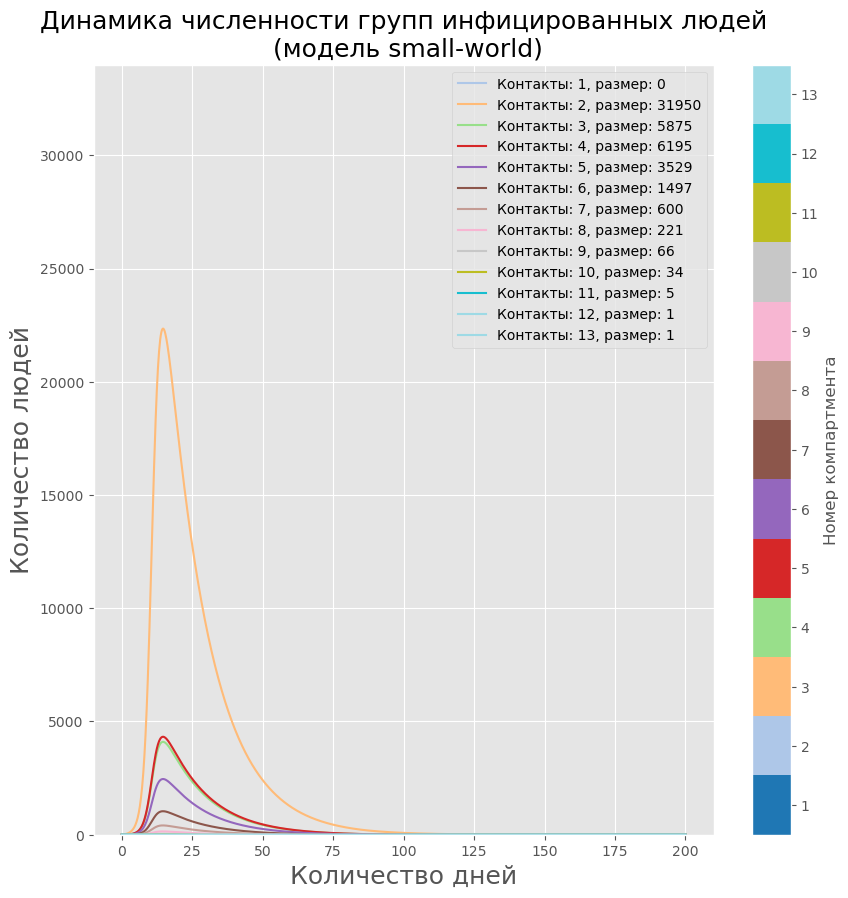
\includegraphics[width=1.0\textwidth]{img/sir_model_small_world_I_rural_new.png}
		\end{minipage}
		\begin{minipage}{0.49\textwidth}
			\centering
			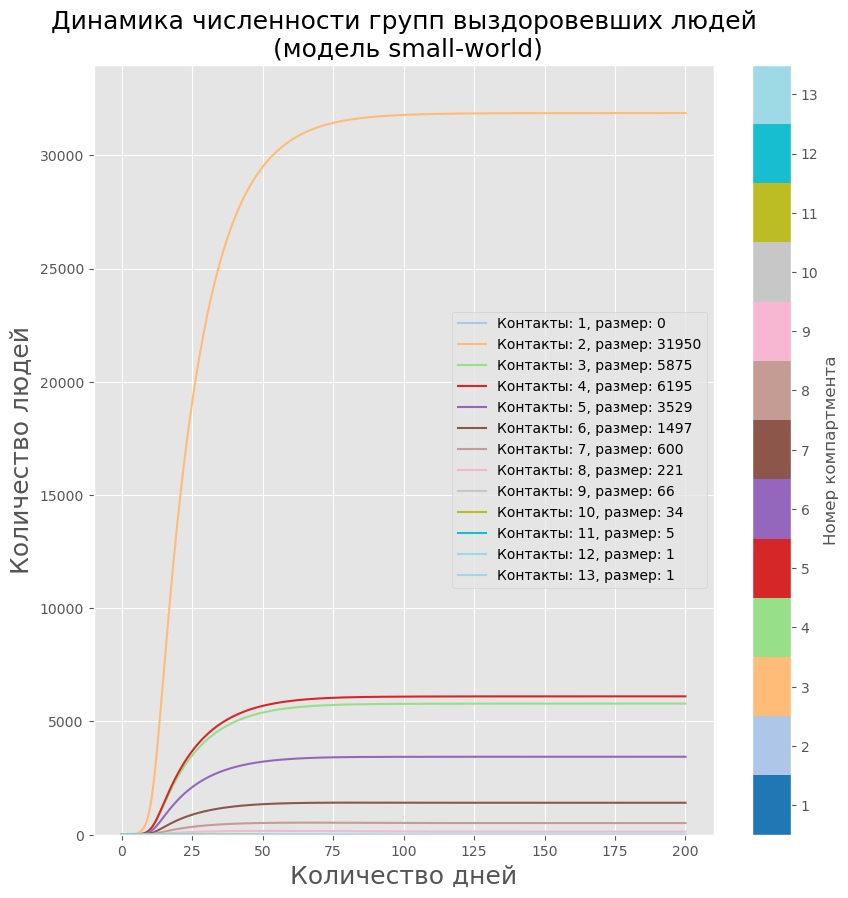
\includegraphics[width=1.0\textwidth]{img/sir_model_small_world_R_rural_new.png}
		\end{minipage}
	\end{figure}
	Динамика изменения размера групп инфицированных и выздоровевших людей с течением времени для сети контактов, полученной с помощью подхода small-world.

	
\end{frame}






\section{\small Результаты}

\begin{comment}
\begin{frame}{Результаты}
	

	\begin{figure}[h!]
		\centering
		\caption{Таблица значений метрик для проведенных в работе экспериментов.}
		\includegraphics[width=1.\textwidth]{img/res.png}
		\label{fig:data}
	\end{figure}
	
	
\end{frame}
\end{comment}


\begin{frame}{Результаты}
	
	
	\begin{enumerate}
		\item Разработан алгоритм построения сети контактов для жителей городской и сельской местностей на основе демографических и социо-эконономических данных о населении Российской Федерации.
		
		\item  Реализована компартментно-сетевая модель для описания распространения респираторной инфекции в популяциях городского и сельского типов.
		
		\item Проведено моделирование распространение инфекции в популяциях с различными типами сетей контактов.
	\end{enumerate}
\end{frame}

\begin{frame}{Выводы}
	\begin{enumerate}
		
		\item Сравнение динамики распространения инфекции для городского и сельского
		населения не выявили серьезных различий. В перспективе, для проведения дополнительного сравнительного анализа распространения
		инфекции в городской и сельской местности можно, например, рассмотреть гипотезу о том, что в сельской местности люди пожилого возраста перестают работать,
		а в городе продолжают.
	
		\item 	Результаты расчётов подтвердили эффективность локдауна, как меры по борьбе с распространением инфекции. В результате эксперимента процент переболевших людей снизился с 74\% до 59\%.
		
		\item При моделировании динамики распространения инфекции на сети контактов small-world необходимо проводить настройку параметра, отвечающего за вероятность переброса ребра в сети контактов.
		
	\end{enumerate}
	
\end{frame}






	
\end{document}
